% !TeX spellcheck = ru_RU
\documentclass[a4paper,12pt]{extarticle}
\usepackage[utf8x]{inputenc}
\usepackage[T1,T2A]{fontenc}
\usepackage[russian]{babel}
\usepackage{hyperref}
\usepackage{indentfirst}
\usepackage{listings}
\usepackage{color}
\usepackage{here}
\usepackage{array}
\usepackage{multirow}
\usepackage{graphicx}

\usepackage{caption}
\renewcommand{\lstlistingname}{Программа} % заголовок листингов кода

\bibliographystyle{ugost2008ls}

\usepackage{listings}
\lstset{ %
extendedchars=\true,
keepspaces=true,
language=C,						% choose the language of the code
basicstyle=\footnotesize,		% the size of the fonts that are used for the code
numbers=left,					% where to put the line-numbers
numberstyle=\footnotesize,		% the size of the fonts that are used for the line-numbers
stepnumber=1,					% the step between two line-numbers. If it is 1 each line will be numbered
numbersep=5pt,					% how far the line-numbers are from the code
backgroundcolor=\color{white},	% choose the background color. You must add \usepackage{color}
showspaces=false				% show spaces adding particular underscores
showstringspaces=false,			% underline spaces within strings
showtabs=false,					% show tabs within strings adding particular underscores
frame=single,           		% adds a frame around the code
tabsize=2,						% sets default tabsize to 2 spaces
captionpos=t,					% sets the caption-position to top
breaklines=true,				% sets automatic line breaking
breakatwhitespace=false,		% sets if automatic breaks should only happen at whitespace
escapeinside={\%*}{*)},			% if you want to add a comment within your code
postbreak=\raisebox{0ex}[0ex][0ex]{\ensuremath{\color{red}\hookrightarrow\space}},
texcl=true,
inputpath=listings,                     % директория с листингами
}

\usepackage[left=2cm,right=2cm,
top=2cm,bottom=2cm,bindingoffset=0cm]{geometry}

%% Нумерация картинок по секциям
\usepackage{chngcntr}
\counterwithin{figure}{section}
\counterwithin{table}{section}

%%Точки нумерации заголовков
\usepackage{titlesec}
\titlelabel{\thetitle.\quad}
\usepackage[dotinlabels]{titletoc}

%% Оформления подписи рисунка
\addto\captionsrussian{\renewcommand{\figurename}{Рисунок}}
\captionsetup[figure]{labelsep = period}

%% Подпись таблицы
\DeclareCaptionFormat{hfillstart}{\hfill#1#2#3\par}
\captionsetup[table]{format=hfillstart,labelsep=newline,justification=centering,skip=-10pt,textfont=bf}

%% Путь к каталогу с рисунками
\graphicspath{{fig/}}

%% Внесение titlepage в учёт счётчика страниц
\makeatletter
\renewenvironment{titlepage} {
 \thispagestyle{empty}
}
\makeatother

\usepackage{minted}

\begin{document}	% начало документа

% Титульная страница
\begin{titlepage}	% начало титульной страницы

	\begin{center}		% выравнивание по центру

		\large Санкт-Петербургский Политехнический Университет Петра Великого\\
		\large Институт компьютерных наук и технологий \\
		\large Кафедра компьютерных систем и программных технологий\\[6cm]
		% название института, затем отступ 6см
		
		\huge Базы данных\\[0.5cm] % название работы, затем отступ 0,5см
		\large Отчет по лабораторной работе №1\\[0.1cm]
		\large Разработка структуры БД\\[5cm]

	\end{center}


	\begin{flushright} % выравнивание по правому краю
		\begin{minipage}{0.25\textwidth} % врезка в половину ширины текста
			\begin{flushleft} % выровнять её содержимое по левому краю

				\large\textbf{Работу выполнил:}\\
				\large Графов Д.И.\\
				\large {Группа:} 33531/2\\
				
				\large \textbf{Преподаватель:}\\
				\large Мяснов А.В.

			\end{flushleft}
		\end{minipage}
	\end{flushright}
	
	\vfill % заполнить всё доступное ниже пространство

	\begin{center}
	\large Санкт-Петербург\\
	\large \the\year % вывести дату
	\end{center} % закончить выравнивание по центру

\thispagestyle{empty} % не нумеровать страницу
\end{titlepage} % конец титульной страницы

\vfill % заполнить всё доступное ниже пространство


\newpage
\setcounter{page}{2}
% Содержание
% Содержание
\renewcommand\contentsname{\centerline{Содержание}}
\tableofcontents
\newpage




\section{Цель работы}
Познакомиться с основами проектирования схемы БД, языком описания сущностей и ограничений БД SQL-DDL.

\section{Программа работы}
	\begin {enumerate}
	\item Самостоятельное изучение SQL-DDL.
	\item Создание скрипта БД в соответствии с согласованной схемой. Должны присутствовать первичные и внешние ключи, ограничения на диапазоны значений. Демонстрация скрипта преподавателю. 
	\item Создание скрипта, заполняющего все таблицы БД данными.
	\item Выполнение SQL-запросов, изменяющих схему созданной БД по заданию преподавателя. Демонстрация их работы преподавателю.
	\end {enumerate}

\section{Теоретическая информация}

\subsection{Язык SQL}
Язык SQL (Structured Query Language) - язык структурированных запросов. Он позволяет формировать весьма сложные запросы к базам данных. В SQL определены два подмножества языка:
\begin {itemize}
	\item SQL-DDL (Data Definition Language) - язык определения структур и ограничений целостности баз данных. Сюда относятся команды создания и удаления баз данных; создания, изменения и удаления таблиц; управления пользователями и т.д.
	\item SQL-DML (Data Manipulation Language) - язык манипулирования данными: добавление, изменение, удаление и извлечение данных, управления транзакциями
\end {itemize}

\subsection{Операции ON DELETE и ON UPDATE}
Выражения ON DELETE и ON UPDATE внешних ключей используются для указания действий, которые будут выполняться при удалении строк родительской таблицы (ON DELETE) или изменении родительского ключа (ON UPDATE). Один и тот же внешний ключ может иметь различные действия, указанные для ON DELETE и ON UPDATE.

В базе данных PostgreSQL действия ON DELETE и ON UPDATE, ассоциированные с внешним ключом, могут быть следующими: NO ACTION, RESTRICT, SET NULL, SET DEFAULT или CASCADE. Если действие не указывается специально, оно по умолчанию является NO ACTION.
Рассмотрим действия, используемые в данной лабораторной работе.

\begin{itemize}
	\item \textbf{NO ACTION}: опция «NO ACTION» означает, что когда родительский ключ изменяется или удаляется из базы данных, никаких специальных действий не производится.
	\item \textbf{CASCADE}: действие «CASCADE» распространяет операции удаления и изменения родительского ключа на зависящие от него дочерние ключи. Для действия ON DELETE CASCADE это выражается в том, что каждая строка дочерней таблицы, которая ассоциирована с удаляемой родительской строкой, также будет удалена. Для действия ON UPDATE CASCADE это выражается в том, что значения, сохранённые в зависящем дочернем ключе, будут заменены на новые значения родительского ключа.
\end{itemize}

\subsection{Типы данных}
Символьные типы данных:
\begin {itemize}
	\item CHAR(n) - символьные строки фиксированной длины. Длина строки определяется параметром n. CHAR без параметра соответствует CHAR(1). Для хранения таких данных всегда отводится n байт вне зависимости от реальной длины строки.
	\item VARCHAR(n) - символьная строка переменной длины. Для хранения данных этого типа отводится число байт, соответствующее реальной длине строки.
\end {itemize}

Целые типы данных:
\begin {itemize}
	\item SMALLINT - короткое целое (2 байта)
	\item INTEGER - обычное целое (4 байта) 
	\item BIGINT - длинное целое (8 байт) 
\end {itemize}

Вещественные типы данных:
\begin {itemize}
	\item REAL - числа с плавающей точкой (4 байта).
	\item DOUBLE PRESCISION - числа с плавающей точкой (8 байт).
	\item NUMERIC(p,n) - тип данных аналогичный FLOAT с числом значащих цифр p и точностью n.
\end {itemize}

Дата и время - используются для хранения даты, времени и их комбинаций:
\begin {itemize}
	\item DATE - тип данных для хранения даты.
	\item TIME - тип данных для хранения времени.
	\item TIMESTAMP - тип данных для хранения моментов времени (год + месяц + день + часы + минуты + секунды + доли секунд).
\end {itemize}

Двоичные типы данных - позволяют хранить данные любого объема в двоичном коде (оцифрованные изображения, исполняемые файлы и т.д.):
\begin {itemize}
	\item BYTEA
\end {itemize}

\section{Выполнение работы}

\subsection {Инициализация}

\begin{center}
	Листинг 1: init.sql
\end{center}
\inputminted[
frame=lines,
framesep=2mm,
baselinestretch=1.2,
fontsize=\footnotesize,
linenos
]{sql}{../src/init.sql}

\subsection {Заполнение}

\begin{center}
	Листинг 2: fill.sql
\end{center}
\inputminted[
frame=lines,
framesep=2mm,
baselinestretch=1.2,
fontsize=\footnotesize,
linenos
]{sql}{../src/fill.sql}

\subsection {Изменение}
Формулировка требуемых изменений:
\begin{enumerate}
	\item Добавить цены на позиции меню в каждом конкретном баре.
	\item Добавить поставки блюд и ингредиентов для коктейлей в бары.
\end{enumerate}

\begin{center}
	Листинг 3: change.sql
\end{center}
\inputminted[
frame=lines,
framesep=2mm,
baselinestretch=1.2,
fontsize=\footnotesize,
linenos
]{sql}{../src/change.sql}

\section {Результат работы}

\begin{figure}[H]
	\begin{center}
		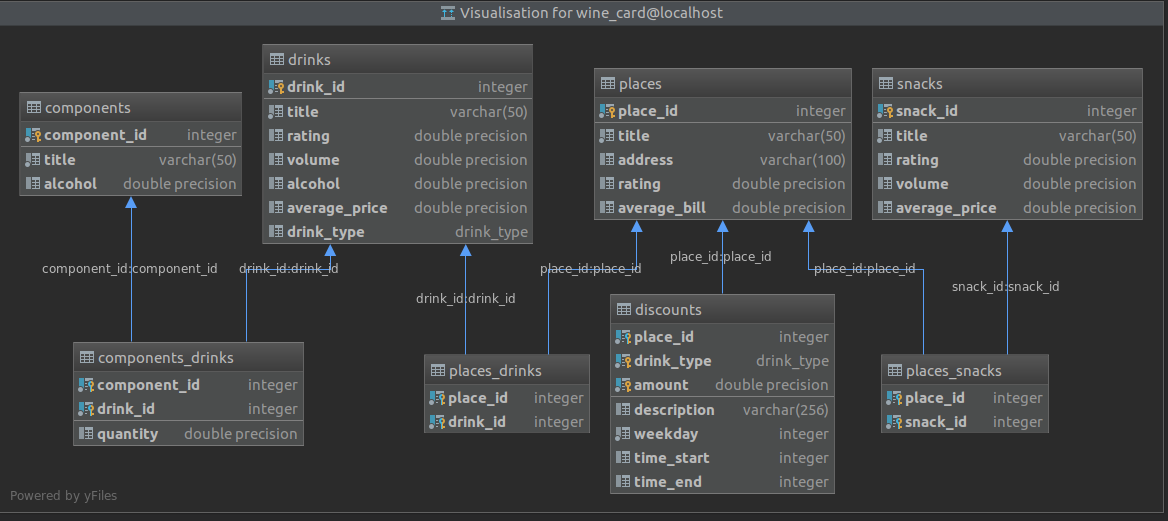
\includegraphics[scale=0.3]{../../structure.png}
		\caption{Структура базы данных} 
		\label{pic:struct} % название для ссылок внутри кода
	\end{center}
\end{figure}

\begin{figure}[H]
	\begin{center}
		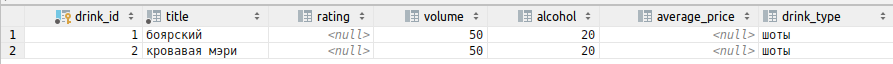
\includegraphics[scale=0.5]{./pics/drinks.png}
		\caption{Содержимое таблицы drinks} 
		\label{pic:drinks} % название для ссылок внутри кода
	\end{center}
\end{figure}

\begin{figure}[H]
	\begin{center}
		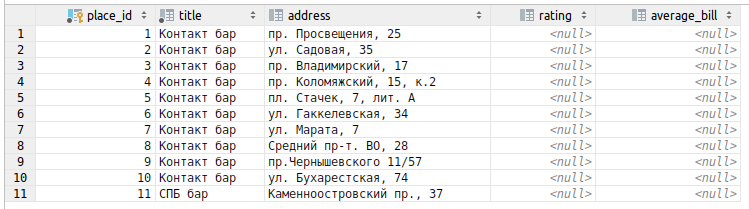
\includegraphics[scale=0.5]{./pics/places.png}
		\caption{Содержимое таблицы places} 
		\label{pic:places} % название для ссылок внутри кода
	\end{center}
\end{figure}

\begin{figure}[H]
	\begin{center}
		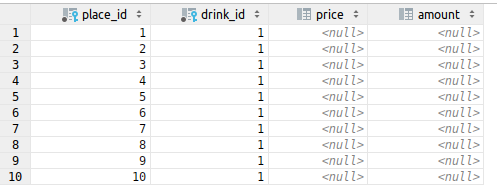
\includegraphics[scale=0.5]{./pics/places_drinks.png}
		\caption{Содержимое таблицы places\_drinks} 
		\label{pic:places_drinks} % название для ссылок внутри кода
	\end{center}
\end{figure}

\newpage
\section{Выводы}

В ходе выполнения данной работы были написаны 3 скрипта на языке PostgreSQL: создающий таблицы; наполняющий таблицы данными; изменяющий таблицы и добавляющий новые.
Таким образом, было осуществлено моё знакомство с основами проектирования схемы БД, языком описания БД SQL-DDL.

\end{document}

